\subsection{Cơ sở dữ liệu}
\subsubsection{Sơ đồ quan hệ thực thế ERD}
\noindent\textbf{Link ERD:} \href{https://viewer.diagrams.net/?tags=%7B%7D\&lightbox=1\&highlight=0000ff\&edit=_blank\&layers=1\&nav=1\&title=%C4%90ATN\&page-id=WVFnYUVKUqSXLER8Fnt_\&dark=auto\#Uhttps%3A%2F%2Fdrive.google.com%2Fuc%3Fid%3D1Dc-fh9fDnhixJ5A2t8bz0mtRvZe8qVRW%26export%3Ddownload}{Mở sơ đồ ERD trên diagrams.net}
\begin{figure}[H]
    \centering
    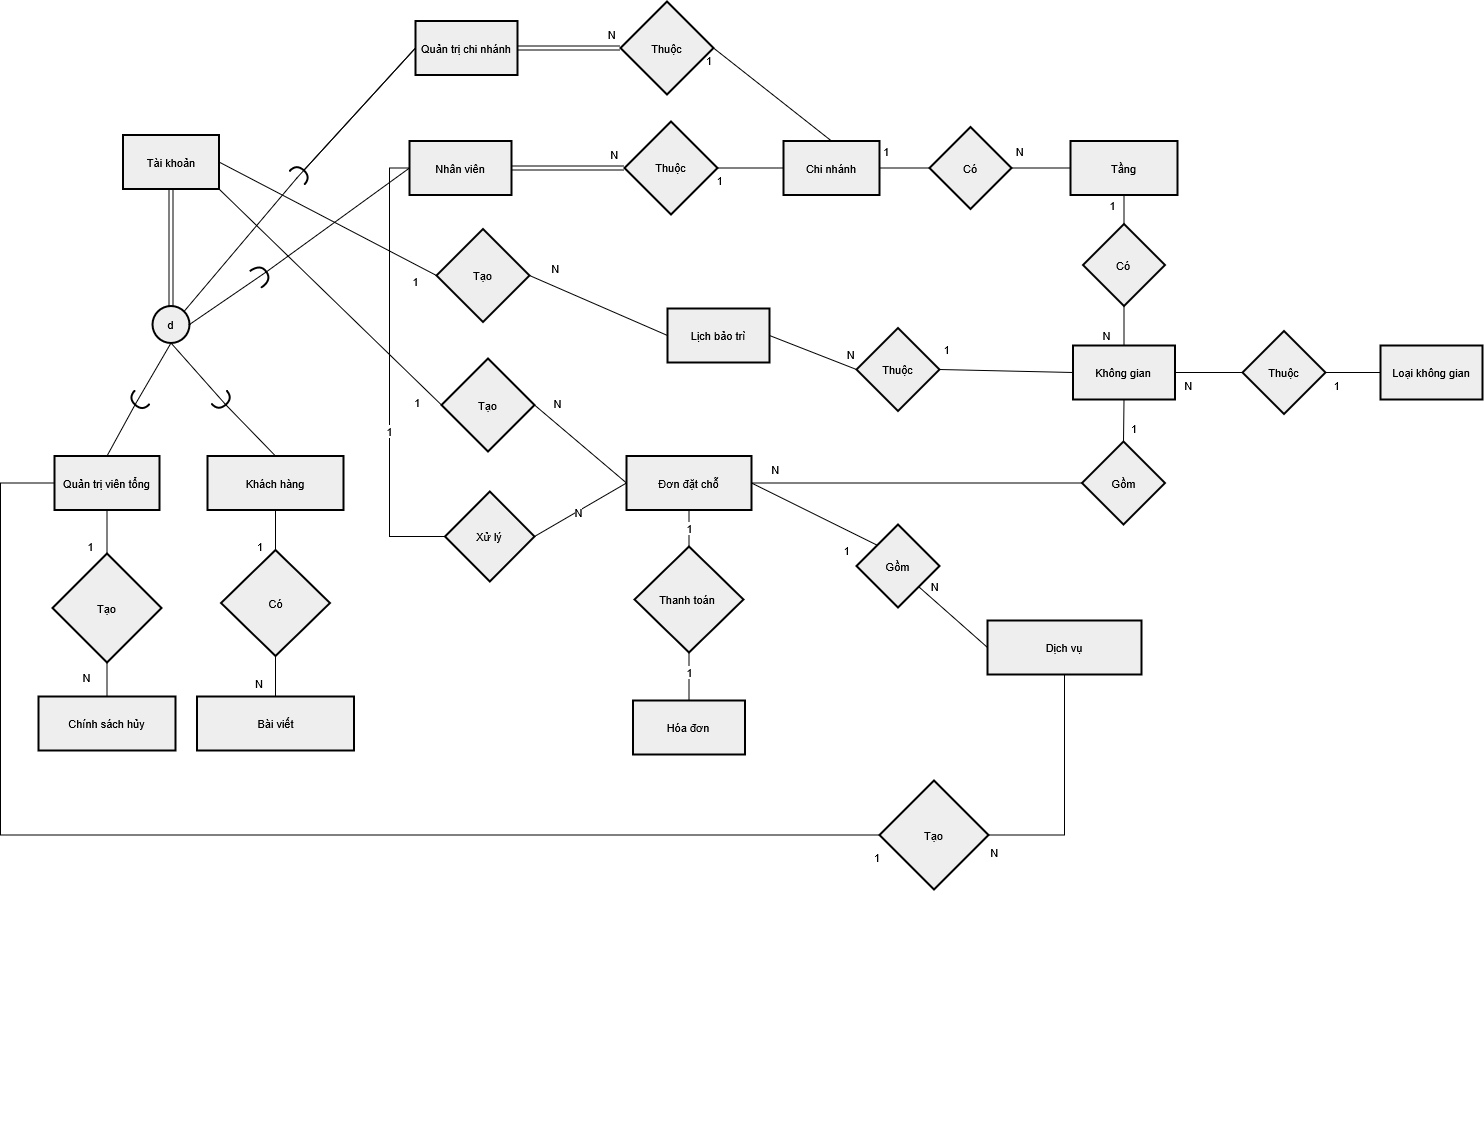
\includegraphics[width=1\textwidth]{Images/Chuong4/ERD.png}
    \caption{Lược đồ thực thể ERD}
    \label{fig:database-erd}
\end{figure}


\subsubsection{Chi tiết các thực thể}

\begin{figure}[H]
    \centering
    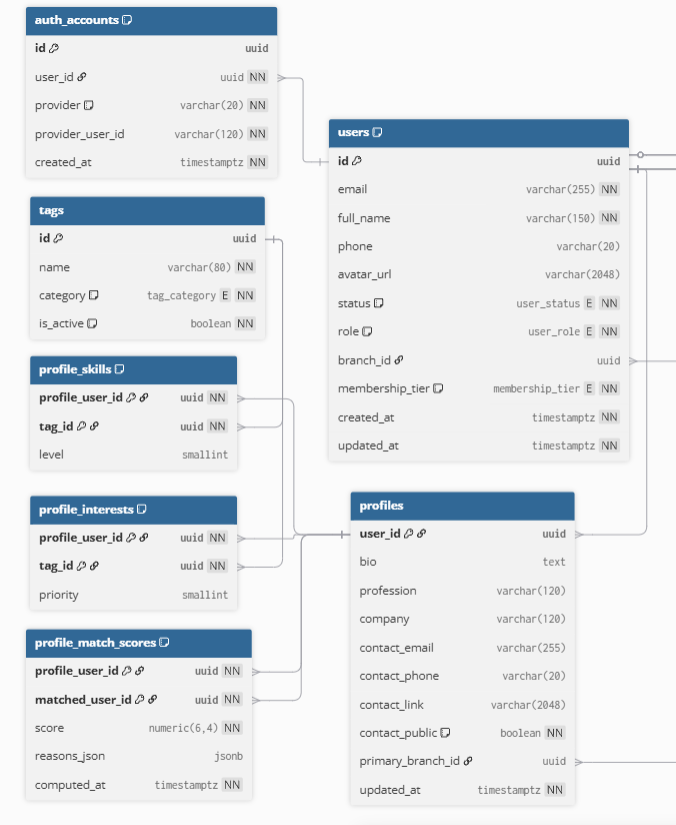
\includegraphics[width=0.8\textwidth]{Images/Chuong4/user_module.png}
    \caption{Sơ đồ module Quản lý người dùng, Xác thực và Gợi ý Kết nối}
    \label{fig:module-user-profile}
\end{figure}

\textbf{Bảng users -- Quản lý người dùng và phân quyền}
\label{table:users}
\begin{longtable}{|p{3cm}|p{2.5cm}|p{3.5cm}|p{5cm}|}
\caption{Bảng users -- Quản lý người dùng và phân quyền} \\
\hline
\textbf{Tên Trường} & \textbf{Kiểu Dữ Liệu} & \textbf{Ràng Buộc} & \textbf{Mô Tả} \\
\hline
\endfirsthead
\hline
\textbf{Tên Trường} & \textbf{Kiểu Dữ Liệu} & \textbf{Ràng Buộc} & \textbf{Mô Tả} \\
\hline
\endhead
id & uuid & PK, NOT NULL & Khóa chính duy nhất của người dùng. \\
\hline
email & varchar(255) & NOT NULL, UNIQUE & Địa chỉ email dùng để đăng nhập và liên lạc, phải là duy nhất. \\
\hline
full\_name & varchar(150) & NOT NULL & Họ và tên đầy đủ. \\
\hline
phone & varchar(20) & & Số điện thoại liên hệ. \\
\hline
avatar\_url & varchar(2048) & & URL dẫn đến ảnh đại diện. \\
\hline
status & user\_status & NOT NULL, DEFAULT 'active' & Trạng thái tài khoản (active, suspended). \\
\hline
role & user\_role & NOT NULL & Vai trò phân quyền (super\_admin, branch\_admin, staff, customer). \\
\hline
branch\_id & uuid & FK to branches.id & ID chi nhánh nhân viên/quản lý trực thuộc. NULL đối với super\_admin và customer. \\
\hline
membership\_tier & membership\_tier & NOT NULL, DEFAULT 'standard' & Cấp độ thành viên của khách hàng (standard, premium). \\
\hline
created\_at & timestamptz & NOT NULL & Thời điểm tạo tài khoản. \\
\hline
updated\_at & timestamptz & NOT NULL & Thời điểm cập nhật thông tin gần nhất. \\
\hline
\end{longtable}

\textbf{Bảng auth\_accounts -- Tài khoản xác thực liên kết}
\label{table:auth_accounts}
\begin{longtable}{|p{3cm}|p{2.5cm}|p{3.5cm}|p{5cm}|}
\caption{Bảng auth\_accounts -- Tài khoản xác thực liên kết} \\
\hline
\textbf{Tên Trường} & \textbf{Kiểu Dữ Liệu} & \textbf{Ràng Buộc} & \textbf{Mô Tả} \\
\hline
\endfirsthead
\hline
\textbf{Tên Trường} & \textbf{Kiểu Dữ Liệu} & \textbf{Ràng Buộc} & \textbf{Mô Tả} \\
\hline
\endhead
id & uuid & PK, NOT NULL & Khóa chính duy nhất của bản ghi xác thực liên kết. \\
\hline
user\_id & uuid & FK to users.id, NOT NULL & ID người dùng sở hữu tài khoản xác thực này. \\
\hline
provider & varchar(20) & NOT NULL & Nhà cung cấp dịch vụ xác thực (ví dụ: 'google'). \\
\hline
provider\_user\_id & varchar(120) & NOT NULL & ID người dùng từ nhà cung cấp dịch vụ bên thứ ba. \\
\hline
created\_at & timestamptz & NOT NULL & Thời điểm liên kết tài khoản. \\
\hline
\end{longtable}

\textbf{Bảng profiles -- Hồ sơ chi tiết người dùng}
\label{table:profiles}
\begin{longtable}{|p{3cm}|p{2.5cm}|p{3.5cm}|p{5cm}|}
\caption{Bảng profiles -- Hồ sơ chi tiết người dùng} \\
\hline
\textbf{Tên Trường} & \textbf{Kiểu Dữ Liệu} & \textbf{Ràng Buộc} & \textbf{Mô Tả} \\
\hline
\endfirsthead
\hline
\textbf{Tên Trường} & \textbf{Kiểu Dữ Liệu} & \textbf{Ràng Buộc} & \textbf{Mô Tả} \\
\hline
\endhead
user\_id & uuid & PK, FK to users.id, NOT NULL & Khóa chính, đồng thời là khóa ngoại liên kết 1-1 với bảng users. \\
\hline
bio & text & & Giới thiệu bản thân ngắn gọn. \\
\hline
profession & varchar(120) & & Nghề nghiệp hoặc chuyên môn của người dùng. \\
\hline
company & varchar(120) & & Tên công ty hoặc tổ chức đang công tác. \\
\hline
contact\_email & varchar(255) & & Email liên hệ công khai được tùy chọn hiển thị. \\
\hline
contact\_phone & varchar(20) & & Số điện thoại liên hệ công khai được tùy chọn hiển thị. \\
\hline
contact\_link & varchar(2048) & & Đường dẫn liên kết cá nhân (LinkedIn, Portfolio, GitHub, v.v.). \\
\hline
contact\_public & boolean & NOT NULL, DEFAULT false & Cờ cho phép hiển thị các thông tin liên hệ công khai cho người dùng khác. \\
\hline
primary\_branch\_id & uuid & FK to branches.id & ID chi nhánh ưu thích hoặc thường xuyên ghé thăm của khách hàng. \\
\hline
updated\_at & timestamptz & NOT NULL & Thời điểm cập nhật hồ sơ gần nhất. \\
\hline
\end{longtable}

\textbf{Bảng tags -- Danh mục thẻ phân loại}
\label{table:tags}
\begin{longtable}{|p{3cm}|p{2.5cm}|p{3.5cm}|p{5cm}|}
\caption{Bảng tags -- Danh mục thẻ phân loại} \\
\hline
\textbf{Tên Trường} & \textbf{Kiểu Dữ Liệu} & \textbf{Ràng Buộc} & \textbf{Mô Tả} \\
\hline
\endfirsthead
\hline
\textbf{Tên Trường} & \textbf{Kiểu Dữ Liệu} & \textbf{Ràng Buộc} & \textbf{Mô Tả} \\
\hline
\endhead
id & uuid & PK, NOT NULL & Khóa chính duy nhất của thẻ. \\
\hline
name & varchar(80) & NOT NULL, UNIQUE & Tên thẻ độc nhất dùng để phân loại (ví dụ: 'React', 'Design', 'Fintech'). \\
\hline
category & tag\_category & NOT NULL, DEFAULT 'skill' & Nhóm phân loại của thẻ (skill, interest, industry). \\
\hline
is\_active & boolean & NOT NULL, DEFAULT true & Cờ xác định thẻ có đang hoạt động hay không. \\
\hline
\end{longtable}

\textbf{Bảng profile\_skills -- Danh sách kỹ năng của hồ sơ}
\label{table:profile_skills}
\begin{longtable}{|p{3cm}|p{2.5cm}|p{3.5cm}|p{5cm}|}
\caption{Bảng profile\_skills -- Danh sách kỹ năng của hồ sơ} \\
\hline
\textbf{Tên Trường} & \textbf{Kiểu Dữ Liệu} & \textbf{Ràng Buộc} & \textbf{Mô Tả} \\
\hline
\endfirsthead
\hline
\textbf{Tên Trường} & \textbf{Kiểu Dữ Liệu} & \textbf{Ràng Buộc} & \textbf{Mô Tả} \\
\hline
\endhead
profile\_user\_id & uuid & PK, FK to profiles.user\_id, NOT NULL & ID người dùng sở hữu kỹ năng này. \\
\hline
tag\_id & uuid & PK, FK to tags.id, NOT NULL & ID của thẻ kỹ năng tương ứng. \\
\hline
level & smallint & & Cấp độ thành thạo của kỹ năng (từ 1 đến 5). \\
\hline
\end{longtable}

\textbf{Bảng profile\_interests -- Danh sách sở thích của hồ sơ}
\label{table:profile_interests}
\begin{longtable}{|p{3cm}|p{2.5cm}|p{3.5cm}|p{5cm}|}
\caption{Bảng profile\_interests -- Danh sách sở thích của hồ sơ} \\
\hline
\textbf{Tên Trường} & \textbf{Kiểu Dữ Liệu} & \textbf{Ràng Buộc} & \textbf{Mô Tả} \\
\hline
\endfirsthead
\hline
\textbf{Tên Trường} & \textbf{Kiểu Dữ Liệu} & \textbf{Ràng Buộc} & \textbf{Mô Tả} \\
\hline
\endhead
profile\_user\_id & uuid & PK, FK to profiles.user\_id, NOT NULL & ID người dùng sở hữu sở thích này. \\
\hline
tag\_id & uuid & PK, FK to tags.id, NOT NULL & ID của thẻ sở thích tương ứng. \\
\hline
priority & smallint & & Mức độ quan tâm/ưu tiên (từ 1 đến 5). \\
\hline
\end{longtable}

\textbf{Bảng profile\_\allowbreak match\_\allowbreak scores -- Điểm gợi ý kết nối}
\label{table:profile_match_scores}
\begin{longtable}{|p{3cm}|p{2.5cm}|p{3.5cm}|p{5cm}|}
\caption{Bảng profile\_\allowbreak match\_\allowbreak scores -- Điểm gợi ý kết nối} \\
\hline
\textbf{Tên Trường} & \textbf{Kiểu Dữ Liệu} & \textbf{Ràng Buộc} & \textbf{Mô Tả} \\
\hline
\endfirsthead
\hline
\textbf{Tên Trường} & \textbf{Kiểu Dữ Liệu} & \textbf{Ràng Buộc} & \textbf{Mô Tả} \\
\hline
\endhead
profile\_user\_id & uuid & PK, FK to profiles.user\_id, NOT NULL & ID người dùng gốc để tính điểm gợi ý. \\
\hline
matched\_user\_id & uuid & PK, FK to profiles.user\_id, NOT NULL & ID người dùng đối tác được gợi ý kết nối. \\
\hline
score & numeric(6,4) & NOT NULL & Điểm số tương đồng tương thích (từ 0.0000 đến 1.0000). \\
\hline
reasons\_json & jsonb & & Lý do chi tiết của gợi ý kết nối dưới dạng tài liệu JSONB. \\
\hline
computed\_at & timestamptz & NOT NULL & Thời điểm thực hiện thuật toán tính điểm kết nối. \\
\hline
\end{longtable}

\begin{figure}[H]
    \centering
    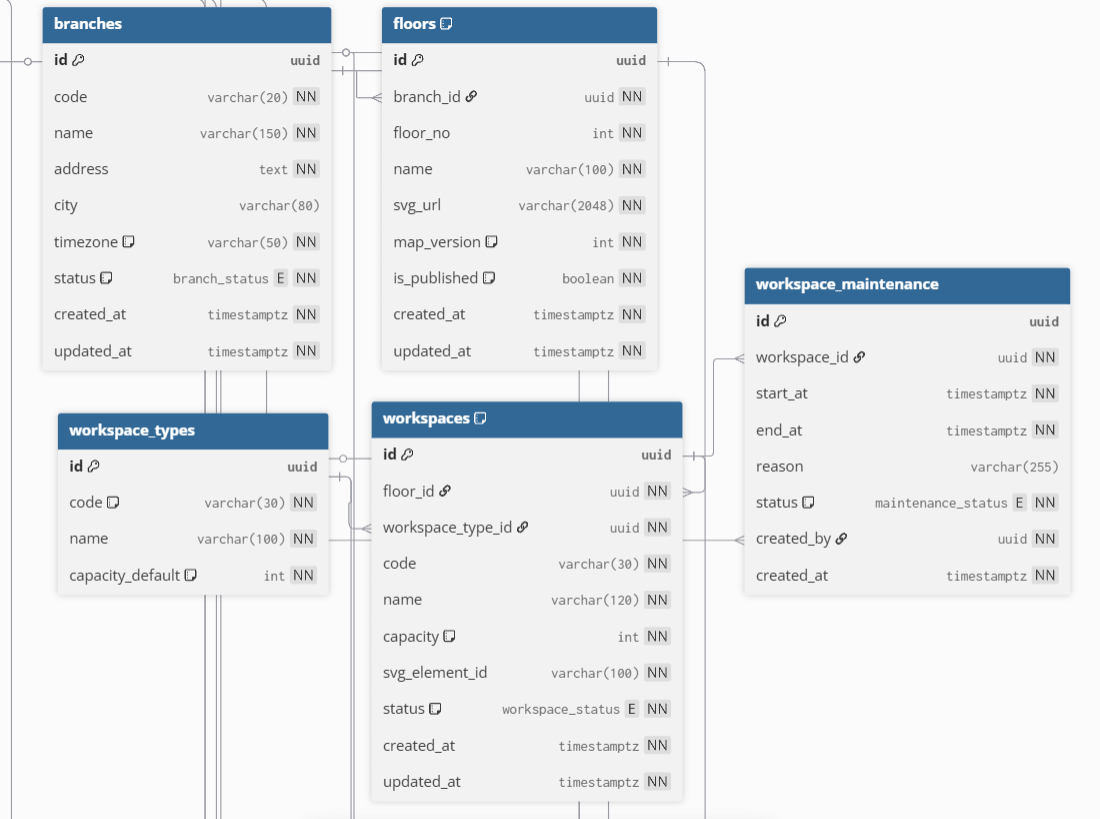
\includegraphics[width=0.8\textwidth]{Images/Chuong4/workspace_module.png}
    \caption{Sơ đồ module Quản lý chi nhánh và không gian làm việc}
    \label{fig:module-branch-workspace}
\end{figure}

\textbf{Bảng branches -- Quản lý chi nhánh co-working space}
\label{table:branches}
\begin{longtable}{|p{3cm}|p{2.5cm}|p{3.5cm}|p{5cm}|}
\caption{Bảng branches -- Quản lý chi nhánh co-working space} \\
\hline
\textbf{Tên Trường} & \textbf{Kiểu Dữ Liệu} & \textbf{Ràng Buộc} & \textbf{Mô Tả} \\
\hline
\endfirsthead
\hline
\textbf{Tên Trường} & \textbf{Kiểu Dữ Liệu} & \textbf{Ràng Buộc} & \textbf{Mô Tả} \\
\hline
\endhead
id & uuid & PK, NOT NULL & Khóa chính duy nhất của chi nhánh. \\
\hline
code & varchar(20) & NOT NULL, UNIQUE & Mã chi nhánh duy nhất (ví dụ: 'HCM-Q1', 'HN-BD'). \\
\hline
name & varchar(150) & NOT NULL & Tên đầy đủ của chi nhánh (ví dụ: 'Văn phòng chi nhánh Quận 1'). \\
\hline
address & text & NOT NULL & Địa chỉ vật lý chi tiết của chi nhánh. \\
\hline
city & varchar(80) & & Thành phố nơi chi nhánh hoạt động. \\
\hline
timezone & varchar(50) & NOT NULL, DEFAULT 'Asia/Ho\_Chi\_Minh' & Múi giờ phục vụ việc đối soát thời gian đặt chỗ chính xác. \\
\hline
status & branch\_status & NOT NULL, DEFAULT 'active' & Trạng thái hoạt động của chi nhánh (active, inactive). \\
\hline
created\_at & timestamptz & NOT NULL & Thời điểm khởi tạo chi nhánh. \\
\hline
updated\_at & timestamptz & NOT NULL & Thời điểm cập nhật chi nhánh gần nhất. \\
\hline
\end{longtable}

\textbf{Bảng floors -- Quản lý các tầng của chi nhánh}
\label{table:floors}
\begin{longtable}{|p{3cm}|p{2.5cm}|p{3.5cm}|p{5cm}|}
\caption{Bảng floors -- Quản lý các tầng của chi nhánh} \\
\hline
\textbf{Tên Trường} & \textbf{Kiểu Dữ Liệu} & \textbf{Ràng Buộc} & \textbf{Mô Tả} \\
\hline
\endfirsthead
\hline
\textbf{Tên Trường} & \textbf{Kiểu Dữ Liệu} & \textbf{Ràng Buộc} & \textbf{Mô Tả} \\
\hline
\endhead
id & uuid & PK, NOT NULL & Khóa chính duy nhất của tầng. \\
\hline
branch\_id & uuid & FK to branches.id, NOT NULL & ID chi nhánh chứa tầng này. \\
\hline
floor\_no & int & NOT NULL & Số thứ tự tầng thực tế (ví dụ: 1, 2, 3, v.v.). \\
\hline
name & varchar(100) & NOT NULL & Tên mô tả của tầng (ví dụ: 'Tầng trệt - Khu vực Hotdesk'). \\
\hline
svg\_url & varchar(2048) & NOT NULL & Đường dẫn URL dẫn tới tệp bản đồ mặt bằng định dạng SVG. \\
\hline
map\_version & int & NOT NULL, DEFAULT 1 & Phiên bản cập nhật của sơ đồ tầng SVG. \\
\hline
is\_published & boolean & NOT NULL, DEFAULT true & Trạng thái công khai của tầng cho khách hàng xem và đặt chỗ. \\
\hline
created\_at & timestamptz & NOT NULL & Thời điểm tạo tầng. \\
\hline
updated\_at & timestamptz & NOT NULL & Thời điểm cập nhật tầng gần nhất. \\
\hline
\end{longtable}

\textbf{Bảng workspace\_\allowbreak types -- Danh mục các loại không gian}
\label{table:workspace_types}
\begin{longtable}{|p{3cm}|p{2.5cm}|p{3.5cm}|p{5cm}|}
\caption{Bảng workspace\_\allowbreak types -- Danh mục các loại không gian} \\
\hline
\textbf{Tên Trường} & \textbf{Kiểu Dữ Liệu} & \textbf{Ràng Buộc} & \textbf{Mô Tả} \\
\hline
\endfirsthead
\hline
\textbf{Tên Trường} & \textbf{Kiểu Dữ Liệu} & \textbf{Ràng Buộc} & \textbf{Mô Tả} \\
\hline
\endhead
id & uuid & PK, NOT NULL & Khóa chính của loại không gian. \\
\hline
code & varchar(30) & NOT NULL, UNIQUE & Mã loại không gian đặc thù (desk: bàn đơn, meeting\_room: phòng họp, private\_office: phòng riêng). \\
\hline
name & varchar(100) & NOT NULL & Tên hiển thị loại không gian. \\
\hline
capacity\_default & int & NOT NULL, DEFAULT 1 & Sức chứa mặc định cho loại không gian này. \\
\hline
\end{longtable}

\textbf{Bảng workspaces -- Quản lý không gian làm việc cụ thể}
\label{table:workspaces}
\begin{longtable}{|p{3cm}|p{2.5cm}|p{3.5cm}|p{5cm}|}
\caption{Bảng workspaces -- Quản lý không gian làm việc cụ thể} \\
\hline
\textbf{Tên Trường} & \textbf{Kiểu Dữ Liệu} & \textbf{Ràng Buộc} & \textbf{Mô Tả} \\
\hline
\endfirsthead
\hline
\textbf{Tên Trường} & \textbf{Kiểu Dữ Liệu} & \textbf{Ràng Buộc} & \textbf{Mô Tả} \\
\hline
\endhead
id & uuid & PK, NOT NULL & Khóa chính duy nhất của không gian làm việc. \\
\hline
floor\_id & uuid & FK to floors.id, NOT NULL & ID tầng chứa không gian này. \\
\hline
workspace\_type\_id & uuid & FK to workspace\_\allowbreak types.id, NOT NULL & ID loại không gian tương ứng. \\
\hline
code & varchar(30) & NOT NULL & Mã ký hiệu vị trí trên tầng (ví dụ: 'D-01', 'MR-02'). \\
\hline
name & varchar(120) & NOT NULL & Tên mô tả chi tiết của không gian. \\
\hline
capacity & int & NOT NULL, DEFAULT 1 & Sức chứa thực tế tối đa của không gian. \\
\hline
svg\_element\_id & varchar(100) & NOT NULL & ID của phần tử tương ứng trên tệp đồ họa sơ đồ SVG của tầng, phục vụ tương tác trên bản đồ. \\
\hline
status & workspace\_status & NOT NULL, DEFAULT 'active' & Trạng thái hiện tại của không gian (active, maintenance, inactive). \\
\hline
created\_at & timestamptz & NOT NULL & Thời điểm tạo không gian làm việc. \\
\hline
updated\_at & timestamptz & NOT NULL & Thời điểm cập nhật thông tin lần cuối. \\
\hline
\end{longtable}

\textbf{Bảng workspace\_\allowbreak maintenance -- Lịch trình bảo trì không gian}
\label{table:workspace_maintenance}
\begin{longtable}{|p{3cm}|p{2.5cm}|p{3.5cm}|p{5cm}|}
\caption{Bảng workspace\_\allowbreak maintenance -- Lịch trình bảo trì không gian} \\
\hline
\textbf{Tên Trường} & \textbf{Kiểu Dữ Liệu} & \textbf{Ràng Buộc} & \textbf{Mô Tả} \\
\hline
\endfirsthead
\hline
\textbf{Tên Trường} & \textbf{Kiểu Dữ Liệu} & \textbf{Ràng Buộc} & \textbf{Mô Tả} \\
\hline
\endhead
id & uuid & PK, NOT NULL & Khóa chính duy nhất của lịch bảo trì. \\
\hline
workspace\_id & uuid & FK to workspaces.id, NOT NULL & ID không gian tiến hành bảo trì. \\
\hline
start\_at & timestamptz & NOT NULL & Thời điểm bắt đầu bảo trì. \\
\hline
end\_at & timestamptz & NOT NULL & Thời điểm kết thúc dự kiến của lịch bảo trì. \\
\hline
reason & varchar(255) & & Lý do hoặc nội dung chi tiết công việc bảo trì. \\
\hline
status & maintenance\_\allowbreak status & NOT NULL, DEFAULT 'scheduled' & Trạng thái bảo trì (scheduled, active, done, canceled). \\
\hline
created\_by & uuid & FK to users.id, NOT NULL & ID của nhân viên tạo lịch bảo trì. \\
\hline
created\_at & timestamptz & NOT NULL & Thời điểm khởi tạo lịch bảo trì trong hệ thống. \\
\end{longtable}

\begin{figure}[H]
    \centering
    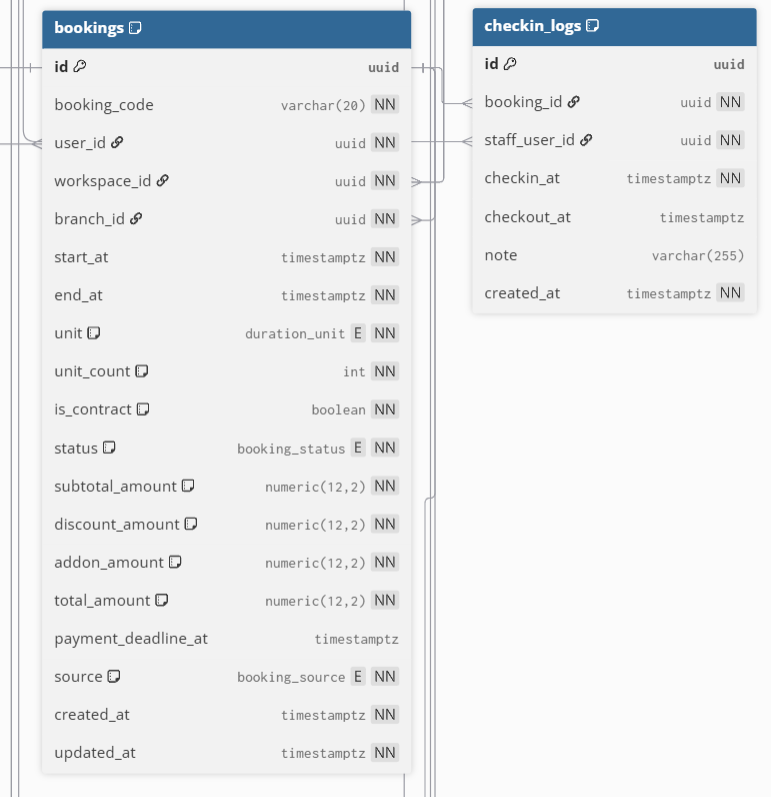
\includegraphics[width=0.8\textwidth]{Images/Chuong4/booking_module.png}
    \caption{Sơ đồ module Quản lý đặt chỗ và check-in}
    \label{fig:module-booking-checkin}
\end{figure}

\textbf{Bảng bookings -- Quản lý thông tin đặt chỗ và hợp đồng}
\label{table:bookings}
\begin{longtable}{|p{3cm}|p{2.5cm}|p{3.5cm}|p{5cm}|}
\caption{Bảng bookings -- Quản lý thông tin đặt chỗ và hợp đồng} \\
\hline
\textbf{Tên Trường} & \textbf{Kiểu Dữ Liệu} & \textbf{Ràng Buộc} & \textbf{Mô Tả} \\
\hline
\endfirsthead
\hline
\textbf{Tên Trường} & \textbf{Kiểu Dữ Liệu} & \textbf{Ràng Buộc} & \textbf{Mô Tả} \\
\hline
\endhead
id & uuid & PK, NOT NULL & Khóa chính duy nhất của lượt đặt chỗ. \\
\hline
booking\_code & varchar(20) & NOT NULL, UNIQUE & Mã đặt chỗ độc nhất gửi đến khách hàng dùng để làm việc và check-in. \\
\hline
user\_id & uuid & FK to users.id, NOT NULL & ID khách hàng thực hiện đặt chỗ. \\
\hline
workspace\_id & uuid & FK to workspaces.id, NOT NULL & ID không gian được đặt. \\
\hline
branch\_id & uuid & FK to branches.id, NOT NULL & ID chi nhánh của không gian, lưu lại để truy vấn nhanh. \\
\hline
start\_at & timestamptz & NOT NULL & Thời điểm bắt đầu của lượt đặt chỗ. \\
\hline
end\_at & timestamptz & NOT NULL & Thời điểm kết thúc của lượt đặt chỗ. \\
\hline
unit & duration\_unit & NOT NULL & Đơn vị thời gian tính tiền đặt chỗ (hour, day, week, month). \\
\hline
unit\_count & int & NOT NULL, DEFAULT 1 & Số lượng đơn vị thời gian thuê. \\
\hline
is\_contract & boolean & NOT NULL, DEFAULT false & Cờ xác định đơn đặt chỗ là hợp đồng thuê dài hạn (tự động bật khi đặt theo week/month). \\
\hline
status & booking\_status & NOT NULL & Trạng thái của đặt chỗ (pending\_payment, confirmed, checked\_in, completed, canceled, expired). \\
\hline
subtotal\_amount & numeric(12,2) & NOT NULL, DEFAULT 0 & Số tiền gốc thuê không gian làm việc. \\
\hline
discount\_amount & numeric(12,2) & NOT NULL, DEFAULT 0 & Số tiền được giảm giá khuyến mãi (nếu có). \\
\hline
addon\_amount & numeric(12,2) & NOT NULL, DEFAULT 0 & Tổng tiền của các dịch vụ bổ sung đi kèm. \\
\hline
total\_amount & numeric(12,2) & NOT NULL, DEFAULT 0 & Tổng số tiền phải thanh toán thực tế (bằng subtotal - discount + addon). \\
\hline
payment\_deadline\_at & timestamptz & & Thời hạn thanh toán cuối cùng (nếu quá giờ chưa thanh toán sẽ tự động hủy). \\
\hline
source & booking\_source & NOT NULL, DEFAULT 'web' & Nguồn khởi tạo đơn đặt chỗ (web, mobile, counter, admin). \\
\hline
created\_at & timestamptz & NOT NULL & Thời điểm tạo đơn đặt chỗ. \\
\hline
updated\_at & timestamptz & NOT NULL & Thời điểm cập nhật đơn hàng gần nhất. \\
\hline
\end{longtable}

\textbf{Bảng checkin\_logs -- Nhật ký check-in và check-out}
\label{table:checkin_logs}
\begin{longtable}{|p{3cm}|p{2.5cm}|p{3.5cm}|p{5cm}|}
\caption{Bảng checkin\_logs -- Nhật ký check-in và check-out} \\
\hline
\textbf{Tên Trường} & \textbf{Kiểu Dữ Liệu} & \textbf{Ràng Buộc} & \textbf{Mô Tả} \\
\hline
\endfirsthead
\hline
\textbf{Tên Trường} & \textbf{Kiểu Dữ Liệu} & \textbf{Ràng Buộc} & \textbf{Mô Tả} \\
\hline
\endhead
id & uuid & PK, NOT NULL & Khóa chính của bản ghi check-in/out. \\
\hline
booking\_id & uuid & FK to bookings.id, NOT NULL & ID đơn đặt chỗ liên quan. \\
\hline
staff\_user\_id & uuid & FK to users.id, NOT NULL & ID nhân viên thực hiện xác nhận check-in/out tại quầy. \\
\hline
checkin\_at & timestamptz & NOT NULL & Thời điểm check-in thực tế của khách hàng. \\
\hline
checkout\_at & timestamptz & & Thời điểm check-out thực tế của khách hàng. \\
\hline
note & varchar(255) & & Ghi chú bổ sung trong quá trình check-in/checkout. \\
\hline
created\_at & timestamptz & NOT NULL & Thời điểm ghi nhận log check-in. \\
\hline
\end{longtable}

\begin{figure}[H]
    \centering
    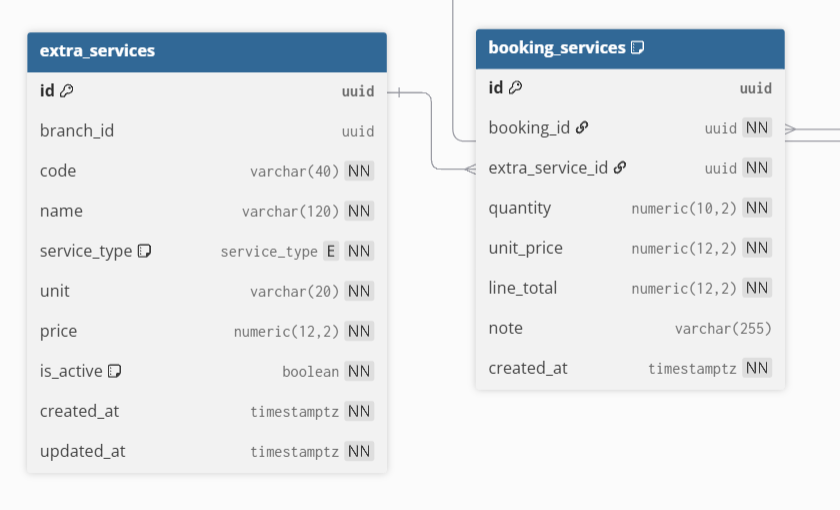
\includegraphics[width=0.8\textwidth]{Images/Chuong4/service_module.png}
    \caption{Sơ đồ module Quản lý dịch vụ bổ sung}
    \label{fig:module-extra-services}
\end{figure}

\textbf{Bảng extra\_services -- Danh mục dịch vụ bổ sung}
\label{table:extra_services}
\begin{longtable}{|p{3cm}|p{2.5cm}|p{3.5cm}|p{5cm}|}
\caption{Bảng extra\_services -- Danh mục dịch vụ bổ sung} \\
\hline
\textbf{Tên Trường} & \textbf{Kiểu Dữ Liệu} & \textbf{Ràng Buộc} & \textbf{Mô Tả} \\
\hline
\endfirsthead
\hline
\textbf{Tên Trường} & \textbf{Kiểu Dữ Liệu} & \textbf{Ràng Buộc} & \textbf{Mô Tả} \\
\hline
\endhead
id & uuid & PK, NOT NULL & Khóa chính của dịch vụ bổ sung. \\
\hline
branch\_id & uuid & FK to branches.id & ID chi nhánh áp dụng riêng cho dịch vụ. NULL nếu là dịch vụ dùng chung trên toàn hệ thống. \\
\hline
code & varchar(40) & NOT NULL, UNIQUE & Mã dịch vụ bổ sung độc nhất. \\
\hline
name & varchar(120) & NOT NULL & Tên hiển thị của dịch vụ (ví dụ: 'Cà phê đá', 'In ấn tài liệu'). \\
\hline
service\_type & service\_type & NOT NULL & Loại hình dịch vụ (drink, meal, printing, other). \\
\hline
unit & varchar(20) & NOT NULL & Đơn vị tính của dịch vụ (ly, phần, trang, v.v.). \\
\hline
price & numeric(12,2) & NOT NULL & Đơn giá áp dụng của dịch vụ. \\
\hline
is\_active & boolean & NOT NULL, DEFAULT true & Trạng thái dịch vụ có đang hoạt động/cung cấp hay không. \\
\hline
created\_at & timestamptz & NOT NULL & Thời điểm khởi tạo dịch vụ. \\
\hline
updated\_at & timestamptz & NOT NULL & Thời điểm cập nhật dịch vụ lần cuối. \\
\hline
\end{longtable}

\textbf{Bảng booking\_services -- Chi tiết sử dụng dịch vụ đi kèm}
\label{table:booking_services}
\begin{longtable}{|p{3cm}|p{2.5cm}|p{3.5cm}|p{5cm}|}
\caption{Bảng booking\_services -- Chi tiết sử dụng dịch vụ đi kèm} \\
\hline
\textbf{Tên Trường} & \textbf{Kiểu Dữ Liệu} & \textbf{Ràng Buộc} & \textbf{Mô Tả} \\
\hline
\endfirsthead
\hline
\textbf{Tên Trường} & \textbf{Kiểu Dữ Liệu} & \textbf{Ràng Buộc} & \textbf{Mô Tả} \\
\hline
\endhead
id & uuid & PK, NOT NULL & Khóa chính duy nhất. \\
\hline
booking\_id & uuid & FK to bookings.id, NOT NULL & ID đơn đặt chỗ sử dụng dịch vụ. \\
\hline
extra\_service\_id & uuid & FK to extra\_services.id, NOT NULL & ID của dịch vụ bổ sung tương ứng. \\
\hline
quantity & numeric(10,2) & NOT NULL & Số lượng dịch vụ sử dụng. \\
\hline
unit\_price & numeric(12,2) & NOT NULL & Đơn giá chụp tại thời điểm đặt chỗ để lưu lại lịch sử giá cố định. \\
\hline
line\_total & numeric(12,2) & NOT NULL & Tổng thành tiền của dòng dịch vụ (bằng quantity * unit\_price). \\
\hline
note & varchar(255) & & Ghi chú thêm (ví dụ: 'Ít đường', 'In 2 mặt'). \\
\hline
created\_at & timestamptz & NOT NULL & Thời điểm ghi nhận dịch vụ vào đơn hàng. \\
\hline
\end{longtable}

\begin{figure}[H]
    \centering
    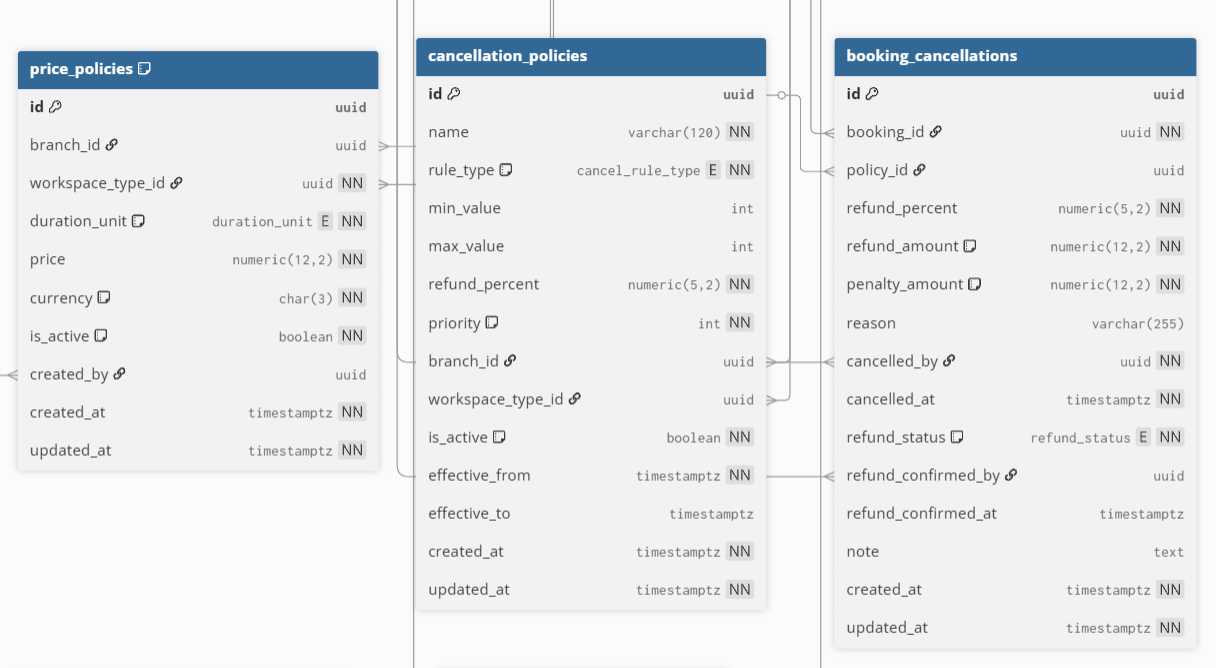
\includegraphics[width=0.8\textwidth]{Images/Chuong4/policy_module.png}
    \caption{Sơ đồ module Quản lý bảng giá và chính sách hủy đặt chỗ}
    \label{fig:module-pricing-policy}
\end{figure}

\textbf{Bảng price\_\allowbreak policies -- Bảng giá thuê không gian}
\label{table:price_policies}
\begin{longtable}{|p{3cm}|p{2.5cm}|p{3.5cm}|p{5cm}|}
\caption{Bảng price\_\allowbreak policies -- Bảng giá thuê không gian} \\
\hline
\textbf{Tên Trường} & \textbf{Kiểu Dữ Liệu} & \textbf{Ràng Buộc} & \textbf{Mô Tả} \\
\hline
\endfirsthead
\hline
\textbf{Tên Trường} & \textbf{Kiểu Dữ Liệu} & \textbf{Ràng Buộc} & \textbf{Mô Tả} \\
\hline
\endhead
id & uuid & PK, NOT NULL & Khóa chính duy nhất của chính sách giá. \\
\hline
branch\_id & uuid & FK to branches.id & ID chi nhánh áp dụng giá override. NULL nếu là chính sách mặc định toàn hệ thống. \\
\hline
workspace\_type\_id & uuid & FK to workspace\_\allowbreak types.id, NOT NULL & ID loại không gian áp dụng bảng giá này. \\
\hline
duration\_unit & duration\_unit & NOT NULL & Đơn vị thời gian tương ứng áp dụng giá (hour, day, week, month). \\
\hline
price & numeric(12,2) & NOT NULL & Giá tiền quy định cho mỗi đơn vị thời gian. \\
\hline
currency & char(3) & NOT NULL, DEFAULT 'VND' & Đơn vị tiền tệ. \\
\hline
is\_active & boolean & NOT NULL, DEFAULT true & Trạng thái hoạt động của chính sách giá. \\
\hline
created\_by & uuid & FK to users.id & ID của người thiết lập chính sách giá này. \\
\hline
created\_at & timestamptz & NOT NULL & Thời điểm tạo chính sách giá. \\
\hline
updated\_at & timestamptz & NOT NULL & Thời điểm cập nhật chính sách giá lần cuối. \\
\end{longtable}

\textbf{Bảng cancellation\_\allowbreak policies -- Danh sách chính sách hủy đặt}
\label{table:cancellation_policies}
\begin{longtable}{|p{3cm}|p{2.5cm}|p{3.5cm}|p{5cm}|}
\caption{Bảng cancellation\_\allowbreak policies -- Danh sách chính sách hủy đặt} \\
\hline
\textbf{Tên Trường} & \textbf{Kiểu Dữ Liệu} & \textbf{Ràng Buộc} & \textbf{Mô Tả} \\
\hline
\endfirsthead
\hline
\textbf{Tên Trường} & \textbf{Kiểu Dữ Liệu} & \textbf{Ràng Buộc} & \textbf{Mô Tả} \\
\hline
\endhead
id & uuid & PK, NOT NULL & Khóa chính duy nhất của chính sách hủy. \\
\hline
name & varchar(120) & NOT NULL & Tên hiển thị chính sách hủy (ví dụ: 'Hủy trước giờ bắt đầu 1 ngày hoàn 100\%'). \\
\hline
rule\_type & cancel\_rule\_type & NOT NULL & Loại quy tắc (GRACE\_HOURS: hủy trong N giờ sau đặt, BEFORE\_START\_DAYS: hủy trước giờ khởi đầu N ngày). \\
\hline
min\_value & int & & Giá trị tối thiểu để thỏa mãn điều kiện chính sách. \\
\hline
max\_value & int & & Giá trị tối đa để thỏa mãn điều kiện chính sách. \\
\hline
refund\_percent & numeric(5,2) & NOT NULL & Tỷ lệ hoàn tiền (từ 0.00\% đến 100.00\%). \\
\hline
priority & int & NOT NULL, DEFAULT 100 & Độ ưu tiên khi áp dụng quy tắc (chính sách ưu tiên cao nhất sẽ được áp dụng trước). \\
\hline
branch\_id & uuid & FK to branches.id & ID chi nhánh áp dụng riêng. NULL nếu áp dụng toàn hệ thống. \\
\hline
workspace\_type\_id & uuid & FK to workspace\_\allowbreak types.id & ID loại không gian áp dụng riêng. NULL nếu áp dụng cho tất cả. \\
\hline
is\_active & boolean & NOT NULL, DEFAULT true & Cờ xác định trạng thái hoạt động của chính sách. \\
\hline
effective\_from & timestamptz & NOT NULL & Thời điểm chính sách bắt đầu có hiệu lực. \\
\hline
effective\_to & timestamptz & & Thời điểm chính sách hết hiệu lực (nếu có). \\
\hline
created\_at & timestamptz & NOT NULL & Thời điểm tạo chính sách. \\
\hline
updated\_at & timestamptz & NOT NULL & Thời điểm cập nhật chính sách lần cuối. \\
\end{longtable}

\textbf{Bảng booking\_\allowbreak cancellations -- Ghi nhận chi tiết lịch sử hủy}
\label{table:booking_cancellations}
\begin{longtable}{|p{3cm}|p{2.5cm}|p{3.5cm}|p{5cm}|}
\caption{Bảng booking\_\allowbreak cancellations -- Ghi nhận chi tiết lịch sử hủy} \\
\hline
\textbf{Tên Trường} & \textbf{Kiểu Dữ Liệu} & \textbf{Ràng Buộc} & \textbf{Mô Tả} \\
\hline
\endfirsthead
\hline
\textbf{Tên Trường} & \textbf{Kiểu Dữ Liệu} & \textbf{Ràng Buộc} & \textbf{Mô Tả} \\
\hline
\endhead
id & uuid & PK, NOT NULL & Khóa chính của bản ghi hủy. \\
\hline
booking\_id & uuid & FK to bookings.id, NOT NULL, UNIQUE & ID đơn đặt chỗ bị hủy (mỗi đơn chỉ hủy 1 lần). \\
\hline
policy\_id & uuid & FK to cancellation\_\allowbreak policies.id & ID chính sách hủy được áp dụng tự động. \\
\hline
refund\_percent & numeric(5,2) & NOT NULL & Tỷ lệ phần trăm hoàn tiền thực tế được áp dụng. \\
\hline
refund\_amount & numeric(12,2) & NOT NULL, DEFAULT 0 & Số tiền hoàn lại cho khách hàng. \\
\hline
penalty\_amount & numeric(12,2) & NOT NULL, DEFAULT 0 & Số tiền phạt khấu trừ từ khách hàng (bằng total\_amount - refund\_amount). \\
\hline
reason & varchar(255) & & Lý do hủy đặt chỗ do khách hàng cung cấp. \\
\hline
cancelled\_by & uuid & FK to users.id, NOT NULL & ID người thực hiện thao tác hủy đặt chỗ. \\
\hline
cancelled\_at & timestamptz & NOT NULL & Thời điểm tiến hành hủy đặt chỗ. \\
\hline
refund\_status & refund\_status & NOT NULL, DEFAULT 'none' & Trạng thái hoàn tiền (none, pending, confirmed, rejected). \\
\hline
refund\_\allowbreak confirmed\_\allowbreak by & uuid & FK to users.id & ID quản trị viên xác nhận đã thanh toán hoàn tiền nội bộ. \\
\hline
refund\_confirmed\_at & timestamptz & & Thời điểm xác nhận hoàn tiền. \\
\hline
note & text & & Ghi chú bổ sung khác về hoàn tiền. \\
\hline
created\_at & timestamptz & NOT NULL & Thời điểm tạo bản ghi hủy đặt chỗ. \\
\hline
updated\_at & timestamptz & NOT NULL & Thời điểm cập nhật bản ghi lần cuối. \\
\end{longtable}

\begin{figure}[H]
    \centering
    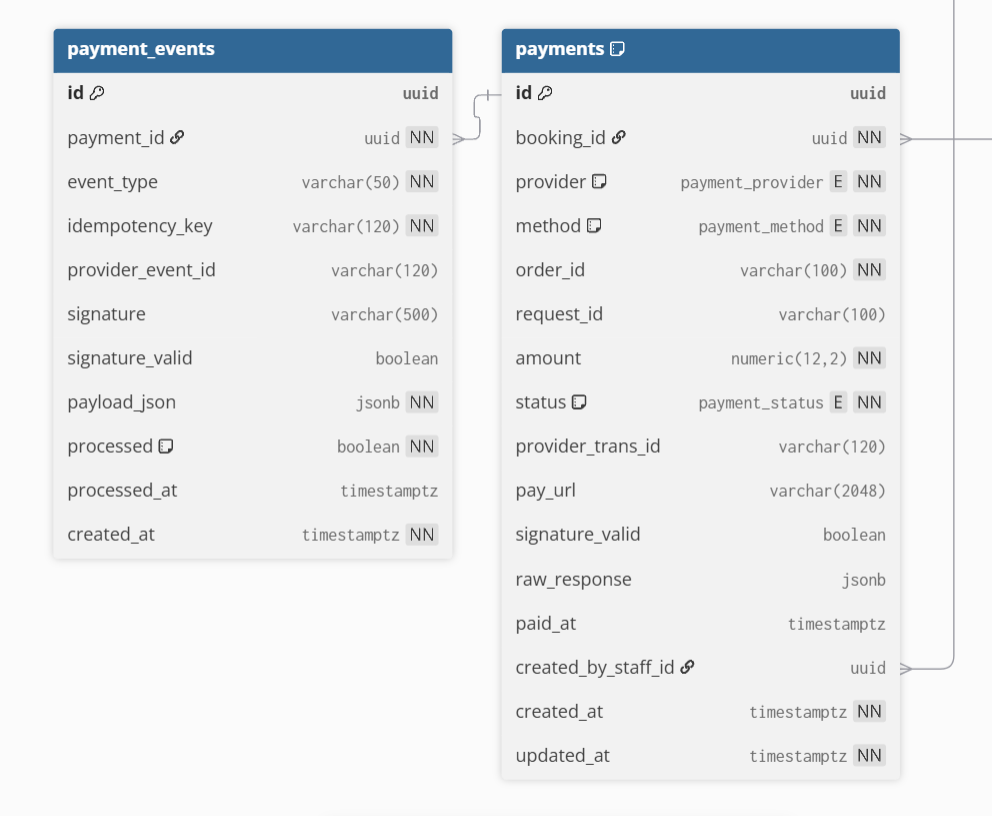
\includegraphics[width=0.8\textwidth]{Images/Chuong4/payment_module.png}
    \caption{Sơ đồ module Quản lý thanh toán}
    \label{fig:module-payment}
\end{figure}

\textbf{Bảng payments -- Ghi nhận giao dịch thanh toán}
\label{table:payments}
\begin{longtable}{|p{3cm}|p{2.5cm}|p{3.5cm}|p{5cm}|}
\caption{Bảng payments -- Ghi nhận giao dịch thanh toán} \\
\hline
\textbf{Tên Trường} & \textbf{Kiểu Dữ Liệu} & \textbf{Ràng Buộc} & \textbf{Mô Tả} \\
\hline
\endfirsthead
\hline
\textbf{Tên Trường} & \textbf{Kiểu Dữ Liệu} & \textbf{Ràng Buộc} & \textbf{Mô Tả} \\
\hline
\endhead
id & uuid & PK, NOT NULL & Khóa chính duy nhất của giao dịch thanh toán. \\
\hline
booking\_id & uuid & FK to bookings.id, NOT NULL & ID đơn đặt chỗ được thanh toán (một đơn đặt có thể có nhiều lần thanh toán thử). \\
\hline
provider & payment\_\allowbreak provider & NOT NULL & Cổng thanh toán (momo, cash). \\
\hline
method & payment\_method & NOT NULL & Phương thức thanh toán chi tiết (ewallet, qr, cash). \\
\hline
order\_id & varchar(100) & NOT NULL, UNIQUE & Mã đơn hàng gửi đến cổng thanh toán dùng để đối soát giao dịch. \\
\hline
request\_id & varchar(100) & & Mã yêu cầu thanh toán đi kèm. \\
\hline
amount & numeric(12,2) & NOT NULL & Số tiền thanh toán của giao dịch. \\
\hline
status & payment\_status & NOT NULL & Trạng thái giao dịch (initiated, pending, paid, failed, expired, canceled, refunded). \\
\hline
provider\_trans\_id & varchar(120) & & Mã giao dịch do cổng thanh toán (MoMo) trả về sau khi giao dịch thành công. \\
\hline
pay\_url & varchar(2048) & & URL dẫn đến trang thanh toán trực tuyến do cổng thanh toán cung cấp. \\
\hline
signature\_valid & boolean & & Kết quả xác thực chữ ký kiểm tra phản hồi từ cổng thanh toán. \\
\hline
raw\_response & jsonb & & Nội dung phản hồi JSONB thô từ cổng thanh toán dùng để lưu lịch sử đối soát lỗi. \\
\hline
paid\_at & timestamptz & & Thời điểm thanh toán thành công. \\
\hline
created\_by\_staff\_id & uuid & FK to users.id & ID nhân viên tại quầy thực hiện xác nhận đã nhận tiền mặt. \\
\hline
created\_at & timestamptz & NOT NULL & Thời điểm tạo giao dịch. \\
\hline
updated\_at & timestamptz & NOT NULL & Thời điểm cập nhật giao dịch gần nhất. \\
\end{longtable}

\textbf{Bảng payment\_events -- Lịch sử sự kiện webhook thanh toán}
\label{table:payment_events}
\begin{longtable}{|p{3cm}|p{2.5cm}|p{3.5cm}|p{5cm}|}
\caption{Bảng payment\_events -- Lịch sử sự kiện webhook thanh toán} \\
\hline
\textbf{Tên Trường} & \textbf{Kiểu Dữ Liệu} & \textbf{Ràng Buộc} & \textbf{Mô Tả} \\
\hline
\endfirsthead
\hline
\textbf{Tên Trường} & \textbf{Kiểu Dữ Liệu} & \textbf{Ràng Buộc} & \textbf{Mô Tả} \\
\hline
\endhead
id & uuid & PK, NOT NULL & Khóa chính duy nhất của sự kiện thanh toán. \\
\hline
payment\_id & uuid & FK to payments.id, NOT NULL & ID giao dịch thanh toán liên quan. \\
\hline
event\_type & varchar(50) & NOT NULL & Tên loại sự kiện nhận được từ webhook (ví dụ: 'momo\_ipn'). \\
\hline
idempotency\_key & varchar(120) & NOT NULL, UNIQUE & Khóa duy nhất dùng để chống xử lý trùng lặp sự kiện webhook từ cổng thanh toán. \\
\hline
provider\_event\_id & varchar(120) & & ID sự kiện từ phía nhà cung cấp thanh toán. \\
\hline
signature & varchar(500) & & Chữ ký đi kèm để kiểm định tính toàn vẹn của sự kiện. \\
\hline
signature\_valid & boolean & & Cờ xác định chữ ký sự kiện webhook có hợp lệ hay không. \\
\hline
payload\_json & jsonb & NOT NULL & Toàn bộ dữ liệu thô (payload) của sự kiện lưu dưới dạng JSONB. \\
\hline
processed & boolean & NOT NULL, DEFAULT false & Trạng thái sự kiện đã được hệ thống xử lý nghiệp vụ hay chưa. \\
\hline
processed\_at & timestamptz & & Thời điểm hoàn tất xử lý sự kiện. \\
\hline
created\_at & timestamptz & NOT NULL & Thời điểm nhận sự kiện webhook vào hệ thống. \\
\end{longtable}

\textbf{Bảng audit\_logs -- Nhật ký kiểm toán hành động hệ thống}
\label{table:audit_logs}
\begin{longtable}{|p{3cm}|p{2.5cm}|p{3.5cm}|p{5cm}|}
\caption{Bảng audit\_logs -- Nhật ký kiểm toán hành động hệ thống} \\
\hline
\textbf{Tên Trường} & \textbf{Kiểu Dữ Liệu} & \textbf{Ràng Buộc} & \textbf{Mô Tả} \\
\hline
\endfirsthead
\hline
\textbf{Tên Trường} & \textbf{Kiểu Dữ Liệu} & \textbf{Ràng Buộc} & \textbf{Mô Tả} \\
\hline
\endhead
id & uuid & PK, NOT NULL & Khóa chính duy nhất của bản ghi log. \\
\hline
actor\_user\_id & uuid & FK to users.id & ID người dùng thực hiện hành động. \\
\hline
actor\_role & varchar(20) & & Vai trò của người thực hiện hành động tại thời điểm ghi log. \\
\hline
action & varchar(100) & NOT NULL & Loại hành động thao tác (ví dụ: 'USER\_LOGIN', 'CREATE\_BOOKING', 'UPDATE\_PRICE'). \\
\hline
target\_table & varchar(60) & NOT NULL & Tên bảng chịu tác động trực tiếp của hành động. \\
\hline
target\_id & uuid & & ID bản ghi chịu tác động trực tiếp. \\
\hline
metadata & jsonb & & Chi tiết thông tin cấu hình thay đổi (giá trị cũ, giá trị mới, IP, trình duyệt) dạng JSONB. \\
\hline
created\_at & timestamptz & NOT NULL & Thời điểm ghi nhận hành động. \\
\end{longtable}

\subsubsection{Mối quan hệ giữa các thực thể}
\label{sec:entity_relationships}

\begin{longtable}{|p{3.2cm}|p{2.8cm}|p{2.8cm}|p{0.9cm}|p{3.6cm}|}
\caption{Mối quan hệ giữa các thực thể} \\
\hline
\textbf{Bảng Nguồn} & \textbf{Khóa Ngoại} & \textbf{Bảng Đích} & \textbf{Loại} & \textbf{Mô Tả} \\
\hline
\endfirsthead
\hline
\textbf{Bảng Nguồn} & \textbf{Khóa Ngoại} & \textbf{Bảng Đích} & \textbf{Loại} & \textbf{Mô Tả} \\
\hline
\endhead
auth\_accounts & user\_id & users & N:1 & Mỗi người dùng có thể có nhiều tài khoản xác thực (như Google SSO). \\
\hline
users & branch\_id & branches & N:1 & Nhiều nhân viên và quản lý thuộc về một chi nhánh nhất định. \\
\hline
profiles & user\_id & users & 1:1 & Mỗi người dùng có một hồ sơ cá nhân duy nhất. \\
\hline
profiles & primary\_branch\_id & branches & N:1 & Chi nhánh yêu thích của người dùng. \\
\hline
profile\_skills & profile\_user\_id & profiles & N:1 & Kỹ năng thuộc về hồ sơ của một người dùng. \\
\hline
profile\_skills & tag\_id & tags & N:1 & Thẻ phân loại kỹ năng tương ứng. \\
\hline
profile\_interests & profile\_user\_id & profiles & N:1 & Sở thích thuộc về hồ sơ của một người dùng. \\
\hline
profile\_interests & tag\_id & tags & N:1 & Thẻ phân loại sở thích tương ứng. \\
\hline
profile\_\allowbreak match\_\allowbreak scores & profile\_user\_id & profiles & N:1 & Hồ sơ người dùng làm đối tượng so khớp gốc. \\
\hline
profile\_\allowbreak match\_\allowbreak scores & matched\_user\_id & profiles & N:1 & Hồ sơ người dùng làm đối tượng được gợi ý. \\
\hline
floors & branch\_id & branches & N:1 & Nhiều tầng thuộc về một chi nhánh nhất định. \\
\hline
workspaces & floor\_id & floors & N:1 & Nhiều không gian làm việc thuộc về một tầng nhất định. \\
\hline
workspaces & workspace\_type\_id & workspace\_\allowbreak types & N:1 & Loại không gian tương ứng. \\
\hline
workspace\_\allowbreak maintenance & workspace\_id & workspaces & N:1 & Lịch bảo trì thuộc về một không gian. \\
\hline
workspace\_\allowbreak maintenance & created\_by & users & N:1 & Người tạo lịch bảo trì là nhân viên/quản lý. \\
\hline
price\_\allowbreak policies & branch\_id & branches & N:1 & Chính sách giá áp dụng riêng cho một chi nhánh (nullable). \\
\hline
price\_\allowbreak policies & workspace\_type\_id & workspace\_\allowbreak types & N:1 & Loại không gian áp dụng giá tương ứng. \\
\hline
price\_\allowbreak policies & created\_by & users & N:1 & Người thiết lập chính sách giá là admin. \\
\hline
bookings & user\_id & users & N:1 & Khách hàng thực hiện đơn đặt chỗ. \\
\hline
bookings & workspace\_id & workspaces & N:1 & Không gian được đặt chỗ. \\
\hline
bookings & branch\_id & branches & N:1 & Chi nhánh của không gian được đặt chỗ. \\
\hline
checkin\_logs & booking\_id & bookings & N:1 & Lượt check-in/out thuộc về một đơn đặt chỗ. \\
\hline
checkin\_logs & staff\_user\_id & users & N:1 & Nhân viên thực hiện xác nhận check-in/out. \\
\hline
payments & booking\_id & bookings & N:1 & Giao dịch thanh toán thuộc về một đơn đặt chỗ. \\
\hline
payments & created\_by\_staff\_id & users & N:1 & Nhân viên quầy xác nhận thanh toán tiền mặt (nullable). \\
\hline
payment\_events & payment\_id & payments & N:1 & Webhook event thuộc về giao dịch thanh toán cụ thể. \\
\hline
cancellation\_\allowbreak policies & branch\_id & branches & N:1 & Chính sách hủy áp dụng riêng cho một chi nhánh. \\
\hline
cancellation\_\allowbreak policies & workspace\_type\_id & workspace\_\allowbreak types & N:1 & Chính sách hủy áp dụng riêng cho một loại không gian. \\
\hline
booking\_\allowbreak cancellations & booking\_id & bookings & 1:1 & Mỗi đơn đặt chỗ chỉ có tối đa một bản ghi hủy đặt. \\
\hline
booking\_\allowbreak cancellations & policy\_id & cancellation\_\allowbreak policies & N:1 & Quy tắc chính sách hủy được áp dụng. \\
\hline
booking\_\allowbreak cancellations & cancelled\_by & users & N:1 & Người thực hiện thao tác hủy đơn đặt chỗ. \\
\hline
booking\_\allowbreak cancellations & refund\_\allowbreak confirmed\_\allowbreak by & users & N:1 & Người xác nhận hoàn tiền thành công. \\
\hline
booking\_services & booking\_id & bookings & N:1 & Chi tiết dịch vụ bổ sung trong đơn đặt. \\
\hline
booking\_services & extra\_service\_id & extra\_services & N:1 & Dịch vụ bổ sung được lựa chọn tương ứng. \\
\hline
audit\_logs & actor\_user\_id & users & N:1 & Nhật ký hành động thuộc về một người dùng thực hiện. \\
\hline
\end{longtable}
% \begin{figure}[H]
%     \centering
%     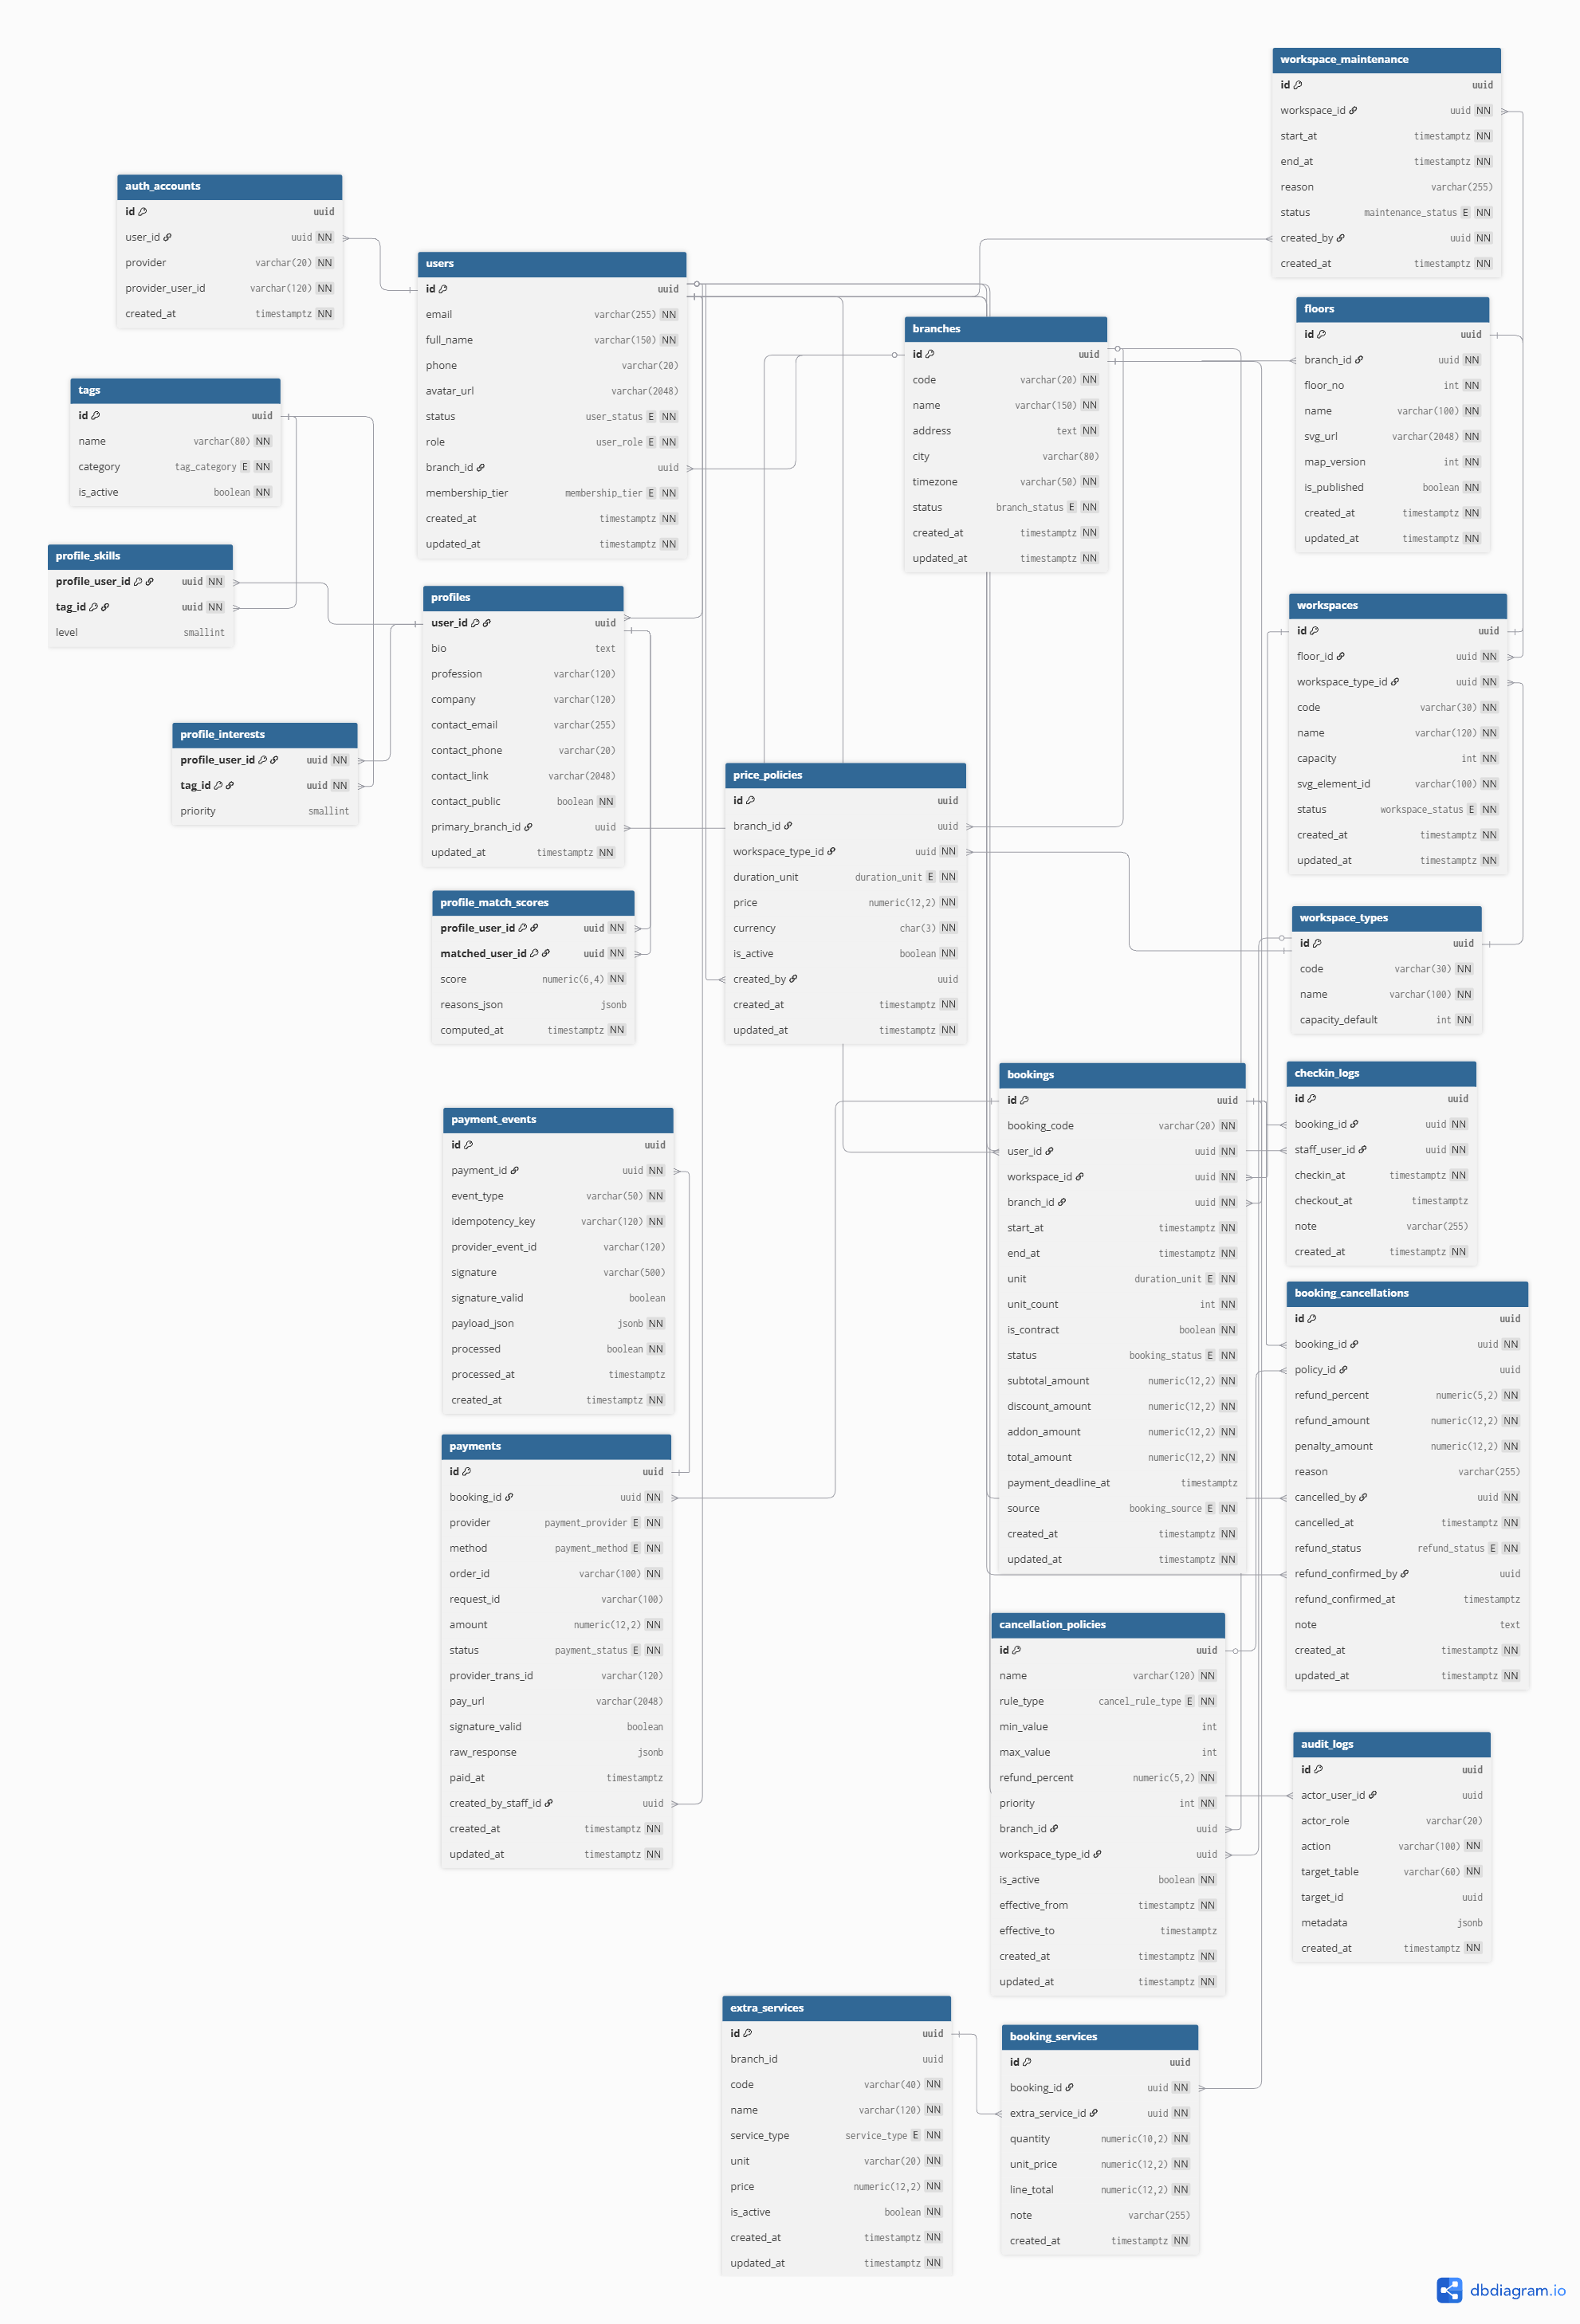
\includegraphics[width=0.8\textwidth]{Images/Chuong4/sodoERD.png}
%     \caption{Sơ đồ tổng quan mối quan hệ giữa các bảng}
%     \label{fig:entity-relationships}
% \end{figure}

